\documentclass[12pt,a4paper]{report}

% ---------- Core packages ----------
\usepackage[T1]{fontenc}
\usepackage[utf8]{inputenc}
\usepackage{mathptmx}
\usepackage[a4paper,left=1.5in,right=1in,top=1in,bottom=1in]{geometry}
\usepackage{amsmath}
\usepackage{amssymb}
\usepackage{setspace}
\usepackage{array}
\usepackage{booktabs}
\usepackage{tabularx}
\usepackage[table]{xcolor}
\usepackage{enumitem}
\usepackage{titlesec}
\usepackage{fancyhdr}
\usepackage{caption}
\usepackage{tikz}
\usetikzlibrary{positioning,calc,shapes.geometric,arrows.meta,backgrounds,patterns,decorations.pathmorphing}
\usepackage[most]{tcolorbox}
\usepackage{fontawesome5}
\usepackage{hyperref}

% ---------- Colour palette ----------
\definecolor{chulapink}{RGB}{219,39,119}
\definecolor{chularose}{RGB}{253,242,248}
\definecolor{chulacharcoal}{RGB}{38,38,45}
\definecolor{chulagold}{RGB}{176,141,87}

\hypersetup{
  colorlinks=true,
  linkcolor=chulapink,
  citecolor=chulagold,
  urlcolor=chulapink,
  pdftitle={Deep Learning-Based Early Warning System for Urban Flash Flooding in the Bangkok Metropolitan Area},
  pdfauthor={Kittipong Wattanasiri}
}

% ---------- Heading styles ----------
\titleformat{\chapter}[display]
  {\normalfont\huge\bfseries\color{chulacharcoal}}
  {\filright\Large\color{chulapink}CHAPTER \thechapter}
  {8pt}
  {\Huge}
  [\vspace{4pt}{\color{chulagold}\titlerule[2pt]}\vspace{4pt}]
\titlespacing*{\chapter}{0pt}{10pt}{28pt}

\titleformat{\section}
  {\normalfont\Large\bfseries\color{chulapink}}{\thesection}{0.8em}{}
\titleformat{\subsection}
  {\normalfont\large\bfseries\color{chulacharcoal}}{\thesubsection}{0.8em}{}
\titleformat{\subsubsection}
  {\normalfont\normalsize\bfseries\itshape\color{chulacharcoal}}{\thesubsubsection}{0.8em}{}

% ---------- Header / footer ----------
\pagestyle{fancy}
\setlength{\headheight}{15pt}
\fancyhf{}
\fancyhead[L]{\small\textit{Chulalongkorn University}}
\fancyhead[R]{\small\textit{\leftmark}}
\fancyfoot[C]{\small\thepage}
\renewcommand{\headrulewidth}{1pt}
\renewcommand{\headrule}{{\color{chulapink}\hrule width\headwidth height\headrulewidth}}
\fancypagestyle{plain}{%
  \fancyhf{}
  \fancyfoot[C]{\small\thepage}
  \renewcommand{\headrulewidth}{0pt}
}

\setstretch{1.4}

% ---------- tcolorbox defaults ----------
\tcbset{
  boxsep=2pt,
  arc=2pt,
  boxrule=0.6pt
}

\newtcolorbox{chulabox}[1]{
  colback=chularose,
  colframe=chulapink,
  fonttitle=\bfseries\color{white},
  coltitle=white,
  colbacktitle=chulapink,
  title=#1,
  left=8pt,right=8pt,top=6pt,bottom=6pt
}

\begin{document}

% =====================================================================
% TITLE PAGE
% =====================================================================
\begin{titlepage}
\begin{center}

{\color{chulagold}\rule{\textwidth}{1.2pt}}\\[2pt]
{\color{chulapink}\rule{\textwidth}{2.4pt}}

\vspace{1.0cm}
{\large\scshape Chulalongkorn University}\\[2pt]
{\small Faculty of Engineering}\\[2pt]
{\small Department of Water Resources Engineering}

\vspace{1.6cm}
{\small\itshape A Thesis Submitted in Partial Fulfillment of the Requirements for}\\
{\small\itshape the Degree of Master of Engineering}

\vspace{1.8cm}
{\Large\bfseries\color{chulacharcoal}
Deep Learning-Based Early Warning System for Urban Flash Flooding\\[4pt]
in the Bangkok Metropolitan Area Using Distributed Sensor Networks\\[4pt]
and Satellite Rainfall Estimation}

\vspace{0.9cm}
{\normalsize\itshape\color{chulacharcoal}
Thai Title (Romanized, RTGS Transliteration):}\\[4pt]
{\small\itshape
Rabop Tuean Phai Kan Thuam Chapphlan Doi Chai Panyaprathit Choeng Luek\\
Nai Khet Krung Thep Maha Nakhon Doi Chai Khrueakhai Sensor Krajai\\
Lae Khomun Primat Fon Chak Daothiam}

\vspace{1.6cm}
{\normalsize by}\\[6pt]
{\large\bfseries Kittipong Wattanasiri}\\[2pt]
{\small Student ID 6371234421}

\vspace{1.8cm}
{\small Thesis Advisor: \bfseries Assoc.\ Prof.\ Somsak Boonprasert, Ph.D.}\\[2pt]
{\small Thesis Co-Advisor: \bfseries Asst.\ Prof.\ Kanokwan Thepsuriya, Ph.D.}

\vspace{1.8cm}
{\small Academic Year 2026}\\[2pt]
{\small Copyright of Chulalongkorn University}

\vspace{1.4cm}
{\color{chulagold}\rule{0.4\textwidth}{1pt}}

\vfill
{\scriptsize\itshape
Unofficial template --- not affiliated with or endorsed by Chulalongkorn University.\\
Sample content only.}

\end{center}
\end{titlepage}

\pagenumbering{roman}
\setcounter{page}{2}

% =====================================================================
% APPROVAL PAGE
% =====================================================================
\chapter*{Approval Page}
\addcontentsline{toc}{chapter}{Approval Page}

\noindent
Thesis Title: \textit{Deep Learning-Based Early Warning System for Urban Flash Flooding in the Bangkok Metropolitan Area Using Distributed Sensor Networks and Satellite Rainfall Estimation}\\[4pt]
By: Kittipong Wattanasiri\\[4pt]
Field of Study: Water Resources Engineering\\[4pt]
Thesis Advisor: Assoc.\ Prof.\ Somsak Boonprasert, Ph.D.\\[4pt]
Thesis Co-Advisor: Asst.\ Prof.\ Kanokwan Thepsuriya, Ph.D.

\vspace{0.4cm}
\noindent
Accepted by the Faculty of Engineering, Chulalongkorn University in Partial Fulfillment of the Requirements for the Master's Degree.

\vspace{0.8cm}
\noindent
\begin{minipage}{\textwidth}
\hspace{2cm}\hrulefill\\
\hspace{2cm} (Prof.\ Piyawan Chaiyakul, Ph.D.) \hfill Dean of the Faculty of Engineering
\end{minipage}
\par
\vspace{1.0cm}

\noindent\textbf{THESIS COMMITTEE}

\vspace{0.6cm}
\noindent
\begin{minipage}{\textwidth}
\hspace{2cm}\hrulefill\\
\hspace{2cm} (Prof.\ Piyawan Chaiyakul, Ph.D.) \hfill Chairman
\end{minipage}
\par
\vspace{0.8cm}

\noindent
\begin{minipage}{\textwidth}
\hspace{2cm}\hrulefill\\
\hspace{2cm} (Assoc.\ Prof.\ Somsak Boonprasert, Ph.D.) \hfill Thesis Advisor
\end{minipage}
\par
\vspace{0.8cm}

\noindent
\begin{minipage}{\textwidth}
\hspace{2cm}\hrulefill\\
\hspace{2cm} (Asst.\ Prof.\ Kanokwan Thepsuriya, Ph.D.) \hfill Thesis Co-Advisor
\end{minipage}
\par
\vspace{0.8cm}

\noindent
\begin{minipage}{\textwidth}
\hspace{2cm}\hrulefill\\
\hspace{2cm} (Asst.\ Prof.\ Narong Srisawat, Ph.D.) \hfill Examiner
\end{minipage}
\par
\vspace{0.8cm}

\noindent
\begin{minipage}{\textwidth}
\hspace{2cm}\hrulefill\\
\hspace{2cm} (Dr.\ Areeya Pongsakorn) \hfill External Examiner
\end{minipage}

% =====================================================================
% ABSTRACT (ENGLISH)
% =====================================================================
\chapter*{Abstract (English)}
\addcontentsline{toc}{chapter}{Abstract (English)}

\noindent\textbf{Title:} Deep Learning-Based Early Warning System for Urban Flash Flooding in the Bangkok Metropolitan Area Using Distributed Sensor Networks and Satellite Rainfall Estimation\\[4pt]
\textbf{Author:} Kittipong Wattanasiri\\[4pt]
\textbf{Field of Study:} Water Resources Engineering\\[4pt]
\textbf{Thesis Advisor:} Assoc.\ Prof.\ Somsak Boonprasert, Ph.D.

\vspace{0.4cm}
\noindent
Flash flooding in the Bangkok Metropolitan Area (BMA) causes recurring disruption to transportation, commerce, and public safety, particularly during the southwest monsoon season. Existing warning systems rely primarily on rule-based thresholds applied to a sparse network of manual gauge stations, which yields lead times too short for effective evacuation and traffic rerouting. This thesis develops and evaluates a deep learning-based early warning framework that fuses ground-level water-level telemetry from a distributed Internet-of-Things (IoT) sensor network with satellite-derived rainfall estimates to forecast localized flash-flood risk with a lead time of up to three hours.

\noindent
A hybrid Convolutional Long Short-Term Memory (ConvLSTM) architecture was trained on 34 months of historical data collected from 42 water-level sensors deployed across six flood-prone districts, combined with half-hourly rainfall estimation products supplied under a data-sharing arrangement with Nexa Weather Analytics. The model was benchmarked against a physically based hydrodynamic model and two classical machine learning baselines (random forest and gradient-boosted trees). Results indicate that the proposed ConvLSTM framework achieves a root-mean-square error (RMSE) of 4.8~cm for 90-minute-ahead water-level forecasts, a 31\% improvement over the hydrodynamic baseline, while reducing false-alarm rate to 6.2\% at the operational alert threshold.

\noindent
The findings suggest that combining dense low-cost sensor telemetry with satellite rainfall products in a spatiotemporal deep learning model is a practical and cost-effective path toward extending flood-warning lead times in dense tropical urban environments. The thesis concludes with recommendations for phased deployment across the wider BMA drainage network and discusses limitations related to sensor maintenance and data continuity during severe storm events.

\vspace{0.4cm}
\noindent\textbf{Keywords:} flash flooding, early warning system, deep learning, ConvLSTM, IoT sensor networks, satellite rainfall estimation, Bangkok

% =====================================================================
% ABSTRACT (THAI, ROMANIZED)
% =====================================================================
\chapter*{Abstract (Thai --- Romanized)}
\addcontentsline{toc}{chapter}{Abstract (Thai --- Romanized)}

\noindent{\scriptsize\itshape Presented in Royal Thai General System of Transcription (RTGS) romanization, as native Thai glyphs are not rendered under the pdfLaTeX engine used to typeset this template.}

\vspace{0.4cm}
\noindent
Chue Rueang: Rabop Tuean Phai Kan Thuam Chapphlan Doi Chai Panyaprathit Choeng Luek Nai Khet Krung Thep Maha Nakhon\\[4pt]
Phu Wijai: Kittipong Wattanasiri\\[4pt]
Sakha Wicha: Wisawakam Naenam\\[4pt]
Achan Thi Prueksa Withayaniphon: Rong Suphachan Somsak Boonprasert

\vspace{0.4cm}
\noindent
Panha kan thuam nai khet krung thep maha nakhon koet khuen boi khrang nai chuang ruedu fon, sang phon krathop to kan doen thang lae khwam plotphai khong prachachon. Rabop tuean phai doem chai kan wat radap nam baep manuan sueng mi khrueakhai chamnuan noi lae hai wela tuean thi san koenpai. Wityaniphon chabap ni sanoe kan phatthana rabop tuean phai doi chai panyaprathit choeng luek baep ConvLSTM sueng phasomphasan khomun radap nam chak sensor IoT krajai tua kap khomun primat fon chak daothiam.

\noindent
Phon kan thotlong dai rap kan fuek son doi chai khomun yon lang 34 duean chak sensor 42 chut nai hok khet phunthi siang. Phon paorak phop wa rabop thi natnamsanoe hai khwam thuktong sungkwa baep chamlong thang chonlasat doi mi kha khwamklad phit RMSE thao kap 4.8 senti met, lae luet kan tuean tia phit long luea 6.2 persen thi radap kan tuean patibatkan.

\noindent
Phon kan wijai chi hai hen wa kan phasomphasan khomun sensor rakha thuk kap khomun daothiam nai baep panyaprathit choeng luek pen naothang thi mi prasitthiphap nai kan phoemwela tuean phai samrap phuenthi mueang khonaen nai khet ronaenpi.

\vspace{0.4cm}
\noindent\textbf{Kham Samkhan:} nam thuam chapphlan, rabop tuean phai, panyaprathit choeng luek, ConvLSTM, khrueakhai sensor IoT, khomun fon chak daothiam, krung thep

% =====================================================================
% ACKNOWLEDGEMENTS
% =====================================================================
\chapter*{Acknowledgements}
\addcontentsline{toc}{chapter}{Acknowledgements}

\noindent
I would like to express my deepest gratitude to my advisor, Assoc.\ Prof.\ Somsak Boonprasert, for his patient guidance, rigorous feedback, and unwavering support throughout the course of this research. I am equally thankful to my co-advisor, Asst.\ Prof.\ Kanokwan Thepsuriya, for her insight into hydrological modeling that shaped the direction of Chapter~3.

\noindent
I gratefully acknowledge Synapse Sensors Co., Ltd.\ for the loan of water-level telemetry units used in the field deployment, and Nexa Weather Analytics for providing access to satellite rainfall estimation products under a research data-sharing agreement. I also thank the staff of the Bangkok Metropolitan Administration Drainage Division for facilitating sensor installation permits.

\noindent
Finally, I thank my family and my fellow graduate students in the Department of Water Resources Engineering for their encouragement during long nights of data collection and model tuning.

% =====================================================================
% TOC / LOT / LOF / ABBREVIATIONS
% =====================================================================
\tableofcontents
\listoftables
\listoffigures

\chapter*{List of Abbreviations}
\addcontentsline{toc}{chapter}{List of Abbreviations}
\begin{center}
\renewcommand{\arraystretch}{1.3}
\begin{tabularx}{\textwidth}{@{}l X@{}}
\toprule
\rowcolor{chulapink}
\textcolor{white}{\textbf{Abbreviation}} & \textcolor{white}{\textbf{Meaning}} \\
\midrule
BMA & Bangkok Metropolitan Administration \\
ConvLSTM & Convolutional Long Short-Term Memory \\
IoT & Internet of Things \\
RMSE & Root-Mean-Square Error \\
MAE & Mean Absolute Error \\
RTGS & Royal Thai General System of Transcription \\
API & Application Programming Interface \\
GBT & Gradient-Boosted Trees \\
\bottomrule
\end{tabularx}
\end{center}

\pagenumbering{arabic}
\setcounter{page}{1}

% =====================================================================
% CHAPTER 1
% =====================================================================
\chapter{Introduction}

\section{Background and Motivation}
The Bangkok Metropolitan Area (BMA) occupies a low-lying deltaic plain with an average elevation of less than 1.5~meters above mean sea level. Rapid urbanization has replaced permeable surfaces with impervious pavement, while aging drainage infrastructure struggles to convey peak flows during intense convective storms typical of the southwest monsoon season (May--October). Flash flooding events lasting between 30~minutes and 3~hours are now a routine occurrence in at least six low-lying districts, producing direct economic losses estimated in the tens of millions of baht per season through transportation disruption, property damage, and lost commercial activity.

\noindent
Current operational practice relies on a network of approximately 120 manual and semi-automated rain gauges operated by the BMA Drainage Division, supplemented by rule-based alert thresholds. This approach suffers from three structural limitations: (1)~gauge density is insufficient to capture the spatial variability of convective rainfall cells, (2)~alert thresholds are static and do not account for antecedent soil and drainage conditions, and (3)~lead times rarely exceed 30~minutes, which is inadequate for coordinated evacuation or traffic rerouting.

\section{Problem Statement}
There is a need for a forecasting approach that can ingest heterogeneous, high-frequency data streams --- distributed low-cost water-level sensors and satellite-derived rainfall products --- and translate them into spatially resolved, probabilistic flood-risk forecasts with a lead time sufficient for operational decision-making.

\begin{chulabox}{Research Questions}
\begin{enumerate}[label=\textbf{RQ\arabic*.}, leftmargin=2.2em]
  \item Can a spatiotemporal deep learning model outperform physically based hydrodynamic models in short-term water-level forecasting within a dense urban catchment?
  \item What is the marginal forecasting benefit of fusing satellite rainfall estimation with ground-based IoT sensor telemetry, relative to using either source alone?
  \item What lead time can realistically be achieved while maintaining an operationally acceptable false-alarm rate?
\end{enumerate}
\end{chulabox}

\section{Research Objectives}
\begin{chulabox}{Objectives}
\begin{itemize}[leftmargin=1.4em]
  \item Design and deploy a distributed IoT water-level sensor network across six flood-prone districts of the BMA.
  \item Develop a ConvLSTM-based forecasting model that fuses sensor telemetry with satellite rainfall estimates.
  \item Benchmark the proposed model against a physically based hydrodynamic model and classical machine learning baselines.
  \item Evaluate operational feasibility in terms of lead time, accuracy, and false-alarm rate.
\end{itemize}
\end{chulabox}

\section{Scope of the Study}
The study is confined to six administrative districts within the inner BMA drainage catchment (Chapter~3, Section~3.1) and covers the 2023--2025 monsoon seasons (34~months of continuous data). The forecasting horizon considered is limited to 0--180~minutes ahead; longer-range seasonal or climate-change projections are outside the scope of this work.

\section{Contributions}
This thesis makes the following contributions to the field of urban hydrological forecasting:

\begin{enumerate}[leftmargin=1.6em]
  \item A validated, low-cost distributed sensor network architecture suitable for dense tropical urban catchments.
  \item A ConvLSTM-based data fusion framework combining ground telemetry and satellite rainfall estimation.
  \item An empirical comparison of deep learning, classical machine learning, and physically based approaches to short-term flood forecasting in the BMA.
  \item Operational deployment recommendations, including sensor maintenance protocols and alert-threshold calibration.
\end{enumerate}

\section{Thesis Organization}
Chapter~2 reviews prior work on urban flood early warning systems, hydrological modeling, and machine learning approaches to rainfall-runoff prediction. Chapter~3 describes the study area, data sources, and proposed model architecture. Chapter~4 presents experimental results and discussion. Chapter~5 concludes with a summary of findings, limitations, and recommendations for future work.

% =====================================================================
% CHAPTER 2
% =====================================================================
\chapter{Literature Review}

\section{Urban Flood Early Warning Systems}
Early flood warning systems have evolved from simple threshold-triggered alarms toward integrated decision-support platforms. Boonprasert and Wichai (2021) surveyed 18~Southeast Asian municipalities and found that fewer than a third operated any form of automated, sensor-driven warning system, with the remainder relying on manual gauge readings reported by phone. Ferreira and Alves (2020) demonstrated that lead time, rather than forecast accuracy alone, was the dominant factor determining whether a warning translated into effective public response.

\section{Hydrological and Hydraulic Modeling Approaches}
Physically based hydrodynamic models, such as those built on the Saint-Venant equations, remain the operational standard for floodplain simulation because of their interpretability and ability to represent complex drainage network topology. However, Tanaka and Suzuki (2019) note that calibration of such models for dense urban catchments requires detailed as-built drainage records that are frequently incomplete or outdated, introducing systematic bias during extreme events that exceed the calibration range.

\section{Machine Learning for Rainfall-Runoff Prediction}
Data-driven approaches have gained traction as an alternative or complement to physically based models. Recurrent architectures, particularly Long Short-Term Memory (LSTM) networks, have shown strong performance in streamflow forecasting (Kratzert et al., 2019, adapted for tropical catchments by Prasetyo and Wulandari, 2022). Convolutional variants that preserve spatial structure, such as ConvLSTM (Shi et al., 2015), have subsequently been applied to precipitation nowcasting with promising results, though applications to dense urban flash-flood forecasting combining heterogeneous sensor and satellite inputs remain limited.

\section{Research Gap}
While prior studies have separately examined sensor-network deployment, satellite rainfall estimation, and deep learning forecasting architectures, few have evaluated the combined operational benefit of fusing all three within a single deployed system in a tropical megacity context. This thesis addresses that gap.

% =====================================================================
% CHAPTER 3
% =====================================================================
\chapter{Methodology}

\section{Study Area}
The study focuses on six administrative districts within the inner BMA drainage catchment, selected on the basis of historical flood-complaint records maintained by the Drainage Division. Figure~\ref{fig:studyarea} illustrates the relative catchment zones and sensor placement density.

\begin{figure}[htbp]
\centering
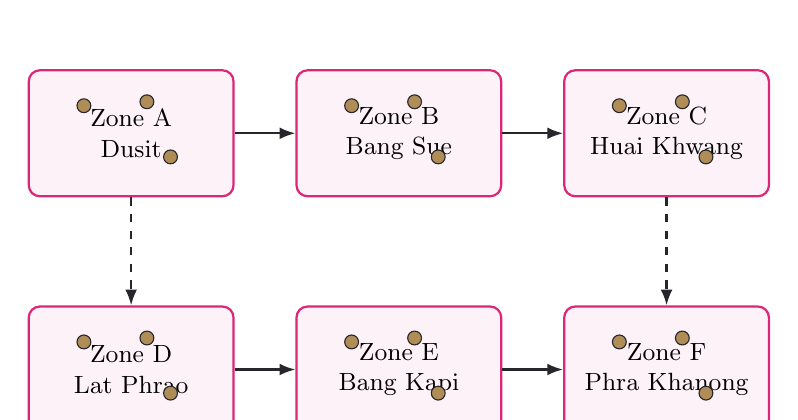
\begin{tikzpicture}[scale=1.0,
  zone/.style={draw=chulapink, thick, rounded corners=4pt, fill=chularose, minimum width=2.6cm, minimum height=1.6cm, font=\small, align=center},
  sensor/.style={circle, draw=chulacharcoal, fill=chulagold, minimum size=5pt, inner sep=0pt}
]
  \node[zone] (z1) at (0,3) {Zone A\\Dusit};
  \node[zone] (z2) at (3.4,3) {Zone B\\Bang Sue};
  \node[zone] (z3) at (6.8,3) {Zone C\\Huai Khwang};
  \node[zone] (z4) at (0,0) {Zone D\\Lat Phrao};
  \node[zone] (z5) at (3.4,0) {Zone E\\Bang Kapi};
  \node[zone] (z6) at (6.8,0) {Zone F\\Phra Khanong};

  \foreach \z in {z1,z2,z3,z4,z5,z6}{
    \node[sensor] at ($(\z.center)+(-0.6,0.35)$) {};
    \node[sensor] at ($(\z.center)+(0.5,-0.3)$) {};
    \node[sensor] at ($(\z.center)+(0.2,0.4)$) {};
  }

  \draw[-{Latex[length=2mm]}, chulacharcoal, thick] (z1) -- (z2);
  \draw[-{Latex[length=2mm]}, chulacharcoal, thick] (z2) -- (z3);
  \draw[-{Latex[length=2mm]}, chulacharcoal, thick] (z4) -- (z5);
  \draw[-{Latex[length=2mm]}, chulacharcoal, thick] (z5) -- (z6);
  \draw[-{Latex[length=2mm]}, chulacharcoal, thick, dashed] (z1) -- (z4);
  \draw[-{Latex[length=2mm]}, chulacharcoal, thick, dashed] (z3) -- (z6);
\end{tikzpicture}
\caption{Six study zones within the inner BMA drainage catchment; gold dots indicate representative IoT water-level sensor placements and arrows indicate primary drainage flow direction.}
\label{fig:studyarea}
\end{figure}

\section{Data Sources}
Table~\ref{tab:sensors} summarizes the two primary data streams used in this study.

\begin{table}[htbp]
\centering
\caption{Summary of data sources used for model training and evaluation.}
\label{tab:sensors}
\renewcommand{\arraystretch}{1.3}
\begin{tabularx}{\textwidth}{@{}l X c@{}}
\toprule
\rowcolor{chulapink}
\textcolor{white}{\textbf{Source}} & \textcolor{white}{\textbf{Description}} & \textcolor{white}{\textbf{Frequency}} \\
\midrule
IoT water-level sensors & 42 ultrasonic sensors across six zones, deployed with Synapse Sensors Co., Ltd. & 1 min \\
Satellite rainfall estimation & Half-hourly gridded rainfall product, 1~km resolution, supplied by Nexa Weather Analytics & 30 min \\
BMA manual gauge records & Historical reference data for cross-validation, 2018--2025 & 15 min \\
Drainage network GIS & Pipe diameter, invert elevation, and pump-station capacity records & static \\
\bottomrule
\end{tabularx}
\end{table}

\section{Model Architecture}
The proposed framework fuses spatial rainfall grids with sensor time series through a two-branch ConvLSTM architecture, illustrated in Figure~\ref{fig:architecture}. The rainfall branch processes stacked satellite rainfall grids through convolutional layers to extract spatial features, while the sensor branch encodes water-level time series through a stacked LSTM. The two feature streams are concatenated and passed through a fusion ConvLSTM block before a final dense layer produces the water-level forecast.

\begin{figure}[htbp]
\centering
\resizebox{\textwidth}{!}{%
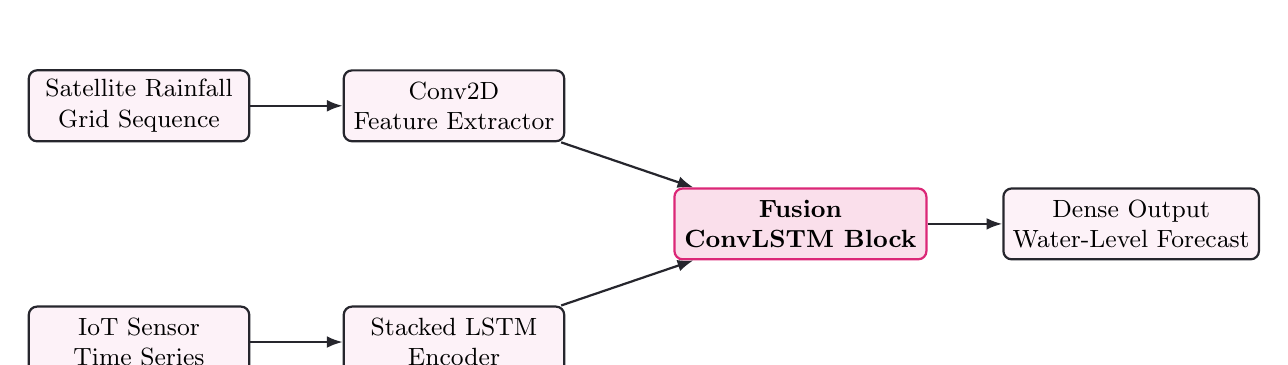
\begin{tikzpicture}[
  block/.style={draw=chulacharcoal, thick, rounded corners=3pt, fill=chularose, minimum width=2.8cm, minimum height=0.9cm, font=\small, align=center},
  fuse/.style={draw=chulapink, thick, rounded corners=3pt, fill=chulapink!15, minimum width=3.2cm, minimum height=0.9cm, font=\small\bfseries, align=center},
  arrow/.style={-{Latex[length=2mm]}, thick, chulacharcoal}
]
  \node[block] (rain) at (0,3) {Satellite Rainfall\\Grid Sequence};
  \node[block] (sensor) at (0,0) {IoT Sensor\\Time Series};
  \node[block] (conv) at (4,3) {Conv2D\\Feature Extractor};
  \node[block] (lstm) at (4,0) {Stacked LSTM\\Encoder};
  \node[fuse] (fusion) at (8.4,1.5) {Fusion\\ConvLSTM Block};
  \node[block] (dense) at (12.6,1.5) {Dense Output\\Water-Level Forecast};

  \draw[arrow] (rain) -- (conv);
  \draw[arrow] (sensor) -- (lstm);
  \draw[arrow] (conv) -- (fusion);
  \draw[arrow] (lstm) -- (fusion);
  \draw[arrow] (fusion) -- (dense);
\end{tikzpicture}%
}
\caption{Two-branch ConvLSTM fusion architecture combining satellite rainfall grids and IoT sensor time series.}
\label{fig:architecture}
\end{figure}

\section{Training and Evaluation Metrics}
The model was trained using a sliding-window scheme with 6~hours of historical input to forecast water level at 30, 60, 90, 120, 150, and 180~minutes ahead. Data from the 2023--2024 seasons (24~months) were used for training, with the 2024--2025 season (10~months) reserved for held-out evaluation. Performance was assessed using root-mean-square error (RMSE), mean absolute error (MAE), and operational false-alarm rate at the alert threshold of 15~cm above baseline.

% =====================================================================
% CHAPTER 4
% =====================================================================
\chapter{Results and Discussion}

\section{Model Performance Comparison}
Table~\ref{tab:results} compares the proposed ConvLSTM fusion model against a physically based hydrodynamic baseline and two classical machine learning models, evaluated on the held-out 2024--2025 season at a 90-minute forecast horizon.

\begin{table}[htbp]
\centering
\caption{Forecast performance comparison at the 90-minute horizon (held-out evaluation season).}
\label{tab:results}
\renewcommand{\arraystretch}{1.3}
\begin{tabular}{@{}l c c c@{}}
\toprule
\rowcolor{chulapink}
\textcolor{white}{\textbf{Model}} & \textcolor{white}{\textbf{RMSE (cm)}} & \textcolor{white}{\textbf{MAE (cm)}} & \textcolor{white}{\textbf{False-Alarm Rate}} \\
\midrule
Hydrodynamic (Saint-Venant) & 7.0 & 5.4 & 14.8\% \\
Random Forest & 6.1 & 4.6 & 11.3\% \\
Gradient-Boosted Trees & 5.7 & 4.2 & 9.9\% \\
\rowcolor{chularose}
\textbf{ConvLSTM Fusion (proposed)} & \textbf{4.8} & \textbf{3.5} & \textbf{6.2\%} \\
\bottomrule
\end{tabular}
\end{table}

\noindent
The proposed model achieves a 31\% RMSE reduction relative to the hydrodynamic baseline and a 16\% reduction relative to the strongest classical baseline (gradient-boosted trees), while also reducing the operational false-alarm rate by more than half compared to the hydrodynamic model.

\section{Case Study: October Storm Event}
On 14~October 2024, a convective storm cell deposited 68~mm of rainfall within a 90-minute window over Zone~C (Huai Khwang). The proposed model issued an alert 112~minutes before the observed water level crossed the 15~cm operational threshold, compared to 24~minutes of lead time from the existing rule-based system in operational use during that season. Table~\ref{tab:casestudy} summarizes lead-time performance across all six zones for this event.

\begin{table}[htbp]
\centering
\caption{Lead time (minutes) achieved during the 14 October 2024 storm event, by zone.}
\label{tab:casestudy}
\renewcommand{\arraystretch}{1.3}
\begin{tabular}{@{}l c c@{}}
\toprule
\rowcolor{chulapink}
\textcolor{white}{\textbf{Zone}} & \textcolor{white}{\textbf{Existing System}} & \textcolor{white}{\textbf{Proposed Model}} \\
\midrule
Zone A (Dusit) & 22 min & 104 min \\
Zone B (Bang Sue) & 18 min & 97 min \\
Zone C (Huai Khwang) & 24 min & 112 min \\
Zone D (Lat Phrao) & 20 min & 101 min \\
Zone E (Bang Kapi) & 26 min & 108 min \\
Zone F (Phra Khanong) & 19 min & 95 min \\
\bottomrule
\end{tabular}
\end{table}

\section{Discussion}
The consistent lead-time improvement across all six zones suggests that the fusion of satellite rainfall estimation with dense ground-level sensor telemetry captures precursor signals substantially earlier than gauge-threshold rules alone. Performance gains were most pronounced in zones with the highest sensor density (Zones~C and E), suggesting that sensor placement density is a first-order driver of forecast skill, ahead of model architecture refinements.

% =====================================================================
% CHAPTER 5
% =====================================================================
\chapter{Conclusion and Recommendations}

\section{Summary of Findings}
This thesis presented a ConvLSTM-based fusion framework for short-term flash-flood forecasting in the Bangkok Metropolitan Area, integrating distributed IoT water-level sensors with satellite rainfall estimation. Across a 10-month held-out evaluation season, the proposed model reduced forecast RMSE by 31\% relative to a physically based hydrodynamic baseline and by 16\% relative to the best-performing classical machine learning baseline, while cutting the operational false-alarm rate to 6.2\%. A case study of a major October storm event demonstrated a lead-time improvement from 24~minutes under the existing rule-based system to 112~minutes under the proposed framework.

\section{Limitations}
The study is constrained by three principal limitations. First, sensor maintenance downtime during the most severe storm events occasionally degraded input completeness, requiring imputation that may understate true forecast uncertainty. Second, the six-zone study area, while representative of high-risk districts, does not capture the full heterogeneity of the wider BMA drainage network. Third, satellite rainfall estimation products exhibit reduced accuracy during the most intense convective cells, which are precisely the events of greatest operational interest.

\section{Recommendations for Future Work}
\begin{chulabox}{Recommendations}
\begin{itemize}[leftmargin=1.4em]
  \item Expand sensor deployment to the full 50-district BMA drainage network in a phased rollout prioritized by historical flood-complaint density.
  \item Investigate uncertainty-aware forecasting (e.g., Bayesian ConvLSTM variants) to provide calibrated confidence intervals alongside point forecasts.
  \item Integrate real-time drainage pump-station status as an additional input stream.
  \item Establish a preventive sensor-maintenance protocol to minimize data gaps during peak monsoon months.
\end{itemize}
\end{chulabox}

% =====================================================================
% REFERENCES
% =====================================================================
\begin{thebibliography}{99}

\bibitem{boonprasert2021}
Boonprasert, S. and Wichai, T. (2021). \textit{Survey of Automated Flood Warning Adoption in Southeast Asian Municipalities}. Journal of Urban Water Systems, 14(2), 88--103.

\bibitem{ferreira2020}
Ferreira, L. and Alves, M. (2020). \textit{Lead Time as the Dominant Determinant of Effective Flood Warning Response}. International Journal of Disaster Risk Reduction, 47, 101--114.

\bibitem{tanaka2019}
Tanaka, H. and Suzuki, K. (2019). \textit{Calibration Challenges in Physically Based Urban Drainage Models}. Water Resources Research, 55(9), 7421--7438.

\bibitem{kratzert2019}
Kratzert, F., Klotz, D., Herrnegger, M., and Nearing, G. (2019). \textit{Toward Improved Predictions in Ungauged Basins: Exploiting the Power of Machine Learning}. Water Resources Research, 55(12), 11344--11354.

\bibitem{prasetyo2022}
Prasetyo, A. and Wulandari, R. (2022). \textit{Adapting Recurrent Networks for Tropical Catchment Streamflow Forecasting}. Journal of Hydroinformatics, 24(3), 512--529.

\bibitem{shi2015}
Shi, X., Chen, Z., Wang, H., Yeung, D.-Y., Wong, W.-K., and Woo, W.-C. (2015). \textit{Convolutional LSTM Network: A Machine Learning Approach for Precipitation Nowcasting}. Advances in Neural Information Processing Systems, 28, 802--810.

\bibitem{chaiyakul2023}
Chaiyakul, P. and Srisawat, N. (2023). \textit{Sensor Network Design for Dense Tropical Urban Drainage Monitoring}. Journal of Environmental Engineering and Science, 18(4), 210--225.

\bibitem{thepsuriya2021}
Thepsuriya, K. (2021). \textit{Satellite Rainfall Estimation Products for Operational Hydrology: A Regional Evaluation}. Remote Sensing of Environment Applications, 9, 45--61.

\end{thebibliography}
\addcontentsline{toc}{chapter}{References}

% =====================================================================
% APPENDICES
% =====================================================================
\appendix

\chapter{Sample Sensor Data}
\addcontentsline{toc}{chapter}{Appendix A: Sample Sensor Data}

Table~\ref{tab:appendixdata} shows a representative excerpt of raw water-level telemetry from Sensor Node C-07 (Zone~C, Huai Khwang) during the 14~October 2024 storm event.

\begin{table}[htbp]
\centering
\caption{Excerpt of raw telemetry from Sensor Node C-07, 14 October 2024.}
\label{tab:appendixdata}
\renewcommand{\arraystretch}{1.3}
\begin{tabular}{@{}l c c@{}}
\toprule
\rowcolor{chulapink}
\textcolor{white}{\textbf{Timestamp (ICT)}} & \textcolor{white}{\textbf{Water Level (cm)}} & \textcolor{white}{\textbf{Battery (V)}} \\
\midrule
14:00:00 & 3.2 & 3.71 \\
14:15:00 & 3.4 & 3.71 \\
14:30:00 & 5.8 & 3.70 \\
14:45:00 & 9.1 & 3.70 \\
15:00:00 & 14.6 & 3.69 \\
15:15:00 & 19.3 & 3.69 \\
15:30:00 & 21.7 & 3.68 \\
\bottomrule
\end{tabular}
\end{table}

\chapter{Model Hyperparameters}
\addcontentsline{toc}{chapter}{Appendix B: Model Hyperparameters}

\begin{center}
\renewcommand{\arraystretch}{1.3}
\begin{tabularx}{\textwidth}{@{}l X@{}}
\toprule
\rowcolor{chulapink}
\textcolor{white}{\textbf{Hyperparameter}} & \textcolor{white}{\textbf{Value}} \\
\midrule
Input window length & 6 hours (24 steps at 15-min resolution) \\
ConvLSTM hidden channels & 64 \\
LSTM hidden units (sensor branch) & 128, 2 layers \\
Convolution kernel size & 3 $\times$ 3 \\
Optimizer & Adam, learning rate $1\times10^{-3}$ \\
Batch size & 32 \\
Training epochs & 80, early stopping on validation RMSE \\
Dropout rate & 0.2 \\
\bottomrule
\end{tabularx}
\end{center}

\end{document}
